\documentclass[a4paper,12pt,twoside]{memoir}

% Castellano
\usepackage[spanish,es-tabla]{babel}
\selectlanguage{spanish}
\usepackage[utf8]{inputenc}
\usepackage[T1]{fontenc}
\usepackage{lmodern} % Scalable font
\usepackage{microtype}
\usepackage{placeins}




\RequirePackage{booktabs}
\RequirePackage[table]{xcolor}
\RequirePackage{xtab}
\RequirePackage{multirow}

% Links
\PassOptionsToPackage{hyphens}{url}\usepackage[colorlinks]{hyperref}
\hypersetup{
	allcolors = {red}
}

% Acrónimos
\usepackage[acronym]{glossaries}
\makenoidxglossaries

\newacronym{llm}{LLM}{\textit{Large Language Models}}
\newacronym{osm}{OSM}{\textit{Open Street Map}}
\newacronym{ods}{ODS}{\textit{Objetivos de Desarrollo Sostenible}}
\newacronym{rag}{RAG}{\textit{Retrieval Augmented Generation}}
\newacronym{ods11}{ODS11}{\textit{Ciudades y Comunidades Sostenibles}}
\newacronym{sdg}{SDG}{\textit{Sustainable Development Goals}}
\newacronym{sc}{Smart City}{\textit{Ciudades Inteligentes}}
\newacronym{sdg11}{SDG11}{\textit{Sustainable Cities and Communities}}
\newacronym{poi}{POI}{\textit{Punto de Interés}}
\newacronym{tfg}{TFG}{\textit{Trabajo de Fin de Grado}}
\newacronym{nlp}{NLP}{\textit{Procesamiento del Lenguaje Natural}}


% Ecuaciones
\usepackage{amsmath}

% Rutas de fichero / paquete
\newcommand{\ruta}[1]{{\sffamily #1}}

% Párrafos
\nonzeroparskip

% Huérfanas y viudas
\widowpenalty100000
\clubpenalty100000

% Imágenes

% Comando para insertar una imagen en un lugar concreto.
% Los parámetros son:
% 1 --> Ruta absoluta/relativa de la figura
% 2 --> Texto a pie de figura
% 3 --> Tamaño en tanto por uno relativo al ancho de página
\usepackage{graphicx}
\newcommand{\imagen}[3]{
	\begin{figure}[!h]
		\centering
		\includegraphics[width=#3\textwidth]{#1}
		\caption{#2}\label{fig:#1}
	\end{figure}
	\FloatBarrier
}

% Comando para insertar una imagen sin posición.
% Los parámetros son:
% 1 --> Ruta absoluta/relativa de la figura
% 2 --> Texto a pie de figura
% 3 --> Tamaño en tanto por uno relativo al ancho de página
\newcommand{\imagenflotante}[3]{
	\begin{figure}
		\centering
		\includegraphics[width=#3\textwidth]{#1}
		\caption{#2}\label{fig:#1}
	\end{figure}
}

% El comando \figura nos permite insertar figuras comodamente, y utilizando
% siempre el mismo formato. Los parametros son:
% 1 --> Porcentaje del ancho de página que ocupará la figura (de 0 a 1)
% 2 --> Fichero de la imagen
% 3 --> Texto a pie de imagen
% 4 --> Etiqueta (label) para referencias
% 5 --> Opciones que queramos pasarle al \includegraphics
% 6 --> Opciones de posicionamiento a pasarle a \begin{figure}
\newcommand{\figuraConPosicion}[6]{%
  \setlength{\anchoFloat}{#1\textwidth}%
  \addtolength{\anchoFloat}{-4\fboxsep}%
  \setlength{\anchoFigura}{\anchoFloat}%
  \begin{figure}[#6]
    \begin{center}%
      \Ovalbox{%
        \begin{minipage}{\anchoFloat}%
          \begin{center}%
            \includegraphics[width=\anchoFigura,#5]{#2}%
            \caption{#3}%
            \label{#4}%
          \end{center}%
        \end{minipage}
      }%
    \end{center}%
  \end{figure}%
}

%
% Comando para incluir imágenes en formato apaisado (sin marco).
\newcommand{\figuraApaisadaSinMarco}[5]{%
  \begin{figure}%
    \begin{center}%
    \includegraphics[angle=90,height=#1\textheight,#5]{#2}%
    \caption{#3}%
    \label{#4}%
    \end{center}%
  \end{figure}%
}
% Para las tablas
\newcommand{\otoprule}{\midrule [\heavyrulewidth]}
%
% Nuevo comando para tablas pequeñas (menos de una página).
\newcommand{\tablaSmall}[5]{%
 \begin{table}
  \begin{center}
   \rowcolors {2}{gray!35}{}
   \begin{tabular}{#2}
    \toprule
    #4
    \otoprule
    #5
    \bottomrule
   \end{tabular}
   \caption{#1}
   \label{tabla:#3}
  \end{center}
 \end{table}
}

%
% Nuevo comando para tablas pequeñas (menos de una página).
\newcommand{\tablaSmallSinColores}[5]{%
 \begin{table}[H]
  \begin{center}
   \begin{tabular}{#2}
    \toprule
    #4
    \otoprule
    #5
    \bottomrule
   \end{tabular}
   \caption{#1}
   \label{tabla:#3}
  \end{center}
 \end{table}
}

\newcommand{\tablaApaisadaSmall}[5]{%
\begin{landscape}
  \begin{table}
   \begin{center}
    \rowcolors {2}{gray!35}{}
    \begin{tabular}{#2}
     \toprule
     #4
     \otoprule
     #5
     \bottomrule
    \end{tabular}
    \caption{#1}
    \label{tabla:#3}
   \end{center}
  \end{table}
\end{landscape}
}

%
% Nuevo comando para tablas grandes con cabecera y filas alternas coloreadas en gris.
\newcommand{\tabla}[6]{%
  \begin{center}
    \tablefirsthead{
      \toprule
      #5
      \otoprule
    }
    \tablehead{
      \multicolumn{#3}{l}{\small\sl continúa desde la página anterior}\\
      \toprule
      #5
      \otoprule
    }
    \tabletail{
      \hline
      \multicolumn{#3}{r}{\small\sl continúa en la página siguiente}\\
    }
    \tablelasttail{
      \hline
    }
    \bottomcaption{#1}
    \rowcolors {2}{gray!35}{}
    \begin{xtabular}{#2}
      #6
      \bottomrule
    \end{xtabular}
    \label{tabla:#4}
  \end{center}
}

%
% Nuevo comando para tablas grandes con cabecera.
\newcommand{\tablaSinColores}[6]{%
  \begin{center}
    \tablefirsthead{
      \toprule
      #5
      \otoprule
    }
    \tablehead{
      \multicolumn{#3}{l}{\small\sl continúa desde la página anterior}\\
      \toprule
      #5
      \otoprule
    }
    \tabletail{
      \hline
      \multicolumn{#3}{r}{\small\sl continúa en la página siguiente}\\
    }
    \tablelasttail{
      \hline
    }
    \bottomcaption{#1}
    \begin{xtabular}{#2}
      #6
      \bottomrule
    \end{xtabular}
    \label{tabla:#4}
  \end{center}
}

%
% Nuevo comando para tablas grandes sin cabecera.
\newcommand{\tablaSinCabecera}[5]{%
  \begin{center}
    \tablefirsthead{
      \toprule
    }
    \tablehead{
      \multicolumn{#3}{l}{\small\sl continúa desde la página anterior}\\
      \hline
    }
    \tabletail{
      \hline
      \multicolumn{#3}{r}{\small\sl continúa en la página siguiente}\\
    }
    \tablelasttail{
      \hline
    }
    \bottomcaption{#1}
  \begin{xtabular}{#2}
    #5
   \bottomrule
  \end{xtabular}
  \label{tabla:#4}
  \end{center}
}



\definecolor{cgoLight}{HTML}{EEEEEE}
\definecolor{cgoExtralight}{HTML}{FFFFFF}

%
% Nuevo comando para tablas grandes sin cabecera.
\newcommand{\tablaSinCabeceraConBandas}[5]{%
  \begin{center}
    \tablefirsthead{
      \toprule
    }
    \tablehead{
      \multicolumn{#3}{l}{\small\sl continúa desde la página anterior}\\
      \hline
    }
    \tabletail{
      \hline
      \multicolumn{#3}{r}{\small\sl continúa en la página siguiente}\\
    }
    \tablelasttail{
      \hline
    }
    \bottomcaption{#1}
    \rowcolors[]{1}{cgoExtralight}{cgoLight}

  \begin{xtabular}{#2}
    #5
   \bottomrule
  \end{xtabular}
  \label{tabla:#4}
  \end{center}
}



\graphicspath{ {./img/} }

% Capítulos
\chapterstyle{bianchi}
\newcommand{\capitulo}[2]{
	\setcounter{chapter}{#1}
	\setcounter{section}{0}
	\setcounter{figure}{0}
	\setcounter{table}{0}
	\chapter*{\thechapter.\enskip #2}
	\addcontentsline{toc}{chapter}{\thechapter.\enskip #2}
	\markboth{#2}{#2}
}

% Apéndices
\renewcommand{\appendixname}{Apéndice}
\renewcommand*\cftappendixname{\appendixname}

\newcommand{\apendice}[1]{
	%\renewcommand{\thechapter}{A}
	\chapter{#1}
}

\renewcommand*\cftappendixname{\appendixname\ }

% Formato de portada
\makeatletter
\usepackage{xcolor}
\newcommand{\tutor}[1]{\def\@tutor{#1}}
\newcommand{\course}[1]{\def\@course{#1}}
\definecolor{cpardoBox}{HTML}{E6E6FF}
\def\maketitle{
  \null
  \thispagestyle{empty}
  % Cabecera ----------------
\noindent
\includegraphics[width=\textwidth]{cabecera}\vspace{1cm}%
  \vfill
  % Título proyecto y escudo informática ----------------
  \colorbox{cpardoBox}{%
    \begin{minipage}{.8\textwidth}
      \vspace{.5cm}\Large
      \begin{center}
      \textbf{TFG del Grado en Ingeniería Informática}\vspace{.6cm}\\
      \textbf{\LARGE\@title{}}
      \end{center}
      \vspace{.2cm}
    \end{minipage}

  }%
  \hfill\begin{minipage}{.20\textwidth}
    
\includegraphics[width=\textwidth]{escudoInfor}
  \end{minipage}
  \vfill
  % Datos de alumno, curso y tutores ------------------
  \begin{center}%
  {%
    \noindent\LARGE
    Presentado por \@author{}\\ 
    en Universidad de Burgos --- \@date{}\\
    Tutor: \@tutor{}\\
  }%
  \end{center}%
  \null
  \cleardoublepage
  }
\makeatother

\newcommand{\nombre}{Fernando Pisot Serrano}


% Datos de portada
\title{\fontsize{14pt}{16pt}\selectfont Aplicación móvil para la generación de rutas turísticas sostenibles basadas en OSM y modelos LLM para promoción de ODS11}
\author{\nombre}
\tutor{Carlos López Nozal}
\date{\today}

\begin{document}

\maketitle


\newpage\null\thispagestyle{empty}\newpage


%%%%%%%%%%%%%%%%%%%%%%%%%%%%%%%%%%%%%%%%%%%%%%%%%%%%%%%%%%%%%%%%%%%%%%%%%%%%%%%%%%%%%%%%
\thispagestyle{empty}


\noindent
\includegraphics[width=\textwidth]{cabecera}\vspace{1cm}

\noindent D. Carlos López Nozal, profesor del departamento de Ingeniería Informática, área de Lenguajes y Sistemas Informáticos.

\noindent Expone:

\noindent Que el alumno D. \nombre, con DNI 70873328R, ha realizado el Trabajo final de Grado en Ingeniería Informática titulado título de TFG. 

\noindent Y que dicho trabajo ha sido realizado por el alumno bajo la dirección del que suscribe, en virtud de lo cual se autoriza su presentación y defensa.

\begin{center} %\large
En Burgos, {\large \today}
\end{center}

\vfill\vfill\vfill

\begin{center}
  Vº. Bº. del Tutor:\\[2cm]
  D. \@tutor{}
  \end{center}


\newpage\null\thispagestyle{empty}\newpage




\frontmatter

% Abstract en castellano
\renewcommand*\abstractname{Resumen}
\begin{abstract}
Se busca construir una aplicación móvil con Flutter que proponga al usuario rutas turísticas, generadas mediante la utilización de modelos de lenguaje de gran escala \acrfull{llm} y el framework \textbf{LangChain}. La ruta turística conectará estos lugares que llamaremos puntos de interés y la información será mostrada al usuario a través de herramientas opensource como \acrfull{osm}.

La aplicación se enfocará en las preferencias del usuario y promocionará rutas optimizadas para ciclistas y peatones, que conecten estos \acrfull{poi} de manera que se fomente la \textbf{movilidad sostenible} en el lugar a visitar.

Esta aplicación se alinea con el concepto de \acrshort{sc}, promoviendo activamente los \acrfull{ods}, con un enfoque particular en el \acrfull{ods11}.


\end{abstract}

\renewcommand*\abstractname{Descriptores}
\begin{abstract}
LLM, LangChain, ODS, ODS11, OSM, Smart City, Flutter, Turismo Sostenible, Movilidad Sostenible
\end{abstract}

\clearpage

% Abstract en inglés
\renewcommand*\abstractname{Abstract}
\begin{abstract}
The goal is to build a mobile application with Flutter that suggests tourist routes to users, generated using large language models \acrfull{llm} and the \textbf{LangChain} framework. The tourist route will connect various locations, referred to as points of interest, and the information will be displayed to the user through open-source tools such as \acrfull{osm}.

The application will focus on user preferences and promote routes optimized for cyclists and pedestrians, connecting these \acrfull{poi} in a way that fosters \textbf{sustainable mobility} in the destination.

This application aligns with the concept of \acrshort{sc}, actively promoting the \acrfull{ods}, with a particular focus on \acrfull{ods11}.
\end{abstract}

\renewcommand*\abstractname{Keywords}
\begin{abstract}
LLM, LangChain, SDGs, SDG11, OSM, Smart City, Flutter, Sustainable Tourism, Sustainable Mobility
\end{abstract}


\clearpage

% Indices
\tableofcontents

\clearpage

\listoffigures

\clearpage

\listoftables
\clearpage

\mainmatter
\capitulo{1}{Introducción}


La creciente urbanización y sus desafíos asociados han destacado la necesidad de desarrollar ciudades más sostenibles e inclusivas. A pesar de los avances en esta promoción, muchas urbes aún enfrentan desafíos significativos en la integración de prácticas sostenibles en la vida cotidiana de sus habitantes. La falta de información accesible y personalizada sobre rutas y actividades que promuevan la movilidad sostenible y el turismo responsable es un problema común. Esta brecha de información impide que tanto residentes como turistas adopten hábitos más sostenibles que beneficien al medio ambiente y a la comunidad local.


Para abordar estos desafíos, se han desarrollado diversas aplicaciones y plataformas que buscan promover la sostenibilidad urbana a través de la tecnología. Por ejemplo, proyectos educativos han integrado los ODS en el aprendizaje basado en problemas universitarios, demostrando que este enfoque no solo facilita la educación sobre los ODS, sino que también motiva a los estudiantes a desarrollar soluciones innovadoras para problemas reales\footnote{Markiegi, U., \& Aldalur, I. (2024). Abordando los Objetivos de Desarrollo Sostenible en el Aprendizaje Basado en Problemas universitario. En Actas de las JENUI - Vol. 9 (pp. 251-254). La Coruña.}\footnote{Markiegi, U., Aldalur, I., \& Perez, A. (2023). Integrando los ODS en el grado de Ingeniería Informática. En Actas de las JENUI - Vol. 8 (pp. 249-256). Granada.}. Estos esfuerzos educativos subrayan la importancia de hacer que los ODS sean más conocidos y comprendidos, fomentando una generación de futuros profesionales comprometidos con la sostenibilidad.


En este contexto, la aplicación móvil que proponemos se alinea con estos esfuerzos al proporcionar una herramienta práctica y accesible para la promoción del ODS 11 y la movilidad sostenible.

En este contexto, el Objetivo de Desarrollo Sostenible (ODS) 11, que se centra en hacer que las ciudades y los asentamientos humanos sean inclusivos, seguros, resilientes y sostenibles, emerge como un pilar fundamental. Según el informe de síntesis de la UNESCO sobre el ODS 11, este objetivo no solo es crucial por sí mismo, sino que actúa como un multiplicador, influyendo indirectamente en la consecución de otros ODS debido a su enfoque integral y transversal\footnote{\href{https://uis.unesco.org/sites/default/files/documents/sdg_11_synthesis_report_2023_v11_0_4.pdf}{UNESCO. (2023). SDG 11 Synthesis Report.}}.

Nuestra aplicación, desarrollada con Flutter, utiliza modelos de lenguaje de gran escala (\acrfull{llm}) y el framework LangChain para generar rutas turísticas personalizadas. Estas rutas conectan puntos de interés (\acrfull{poi}) y se visualizan mediante herramientas open-source como \acrfull{osm}.

La aplicación se enfoca en las preferencias del usuario, ofreciendo rutas optimizadas para ciclistas y peatones, y promoviendo así la movilidad sostenible. Al integrar datos y tecnología avanzada, nuestra solución no solo facilita una experiencia turística enriquecedora, sino que también fomenta prácticas sostenibles que pueden tener un impacto positivo en la comunidad y el medio ambiente.

\end{document}
\capitulo{2}{Objetivos del proyecto}

\section{Objetivos funcionales}

Estos objetivos se centran en las funcionalidades y características que debe tener la aplicación \textit{Eco City Tours} para satisfacer las necesidades y expectativas de los usuarios. A continuación se detallan los objetivos funcionales del proyecto:

\begin{itemize}
    \item \textbf{Propuesta de rutas turísticas personalizadas}: La aplicación debe ser capaz de generar rutas turísticas personalizadas basadas en las preferencias del visitante utilizando \acrfull{llm}. Para llevarlo a cabo, el usuario facilitará al modelo sus preferencias, eligiendo entre otras opciones el medio de transporte elegido o el número de \acrfull{pdi} a visitar.
    \item \textbf{Obtener los \acrfull{pdi}}: A través de la interacción con el modelo \acrshort{llm}, la aplicación le indicará que debe priorizar un \acrshort{pdi} sobre otro en función de criterios sostenibles como la deslocalización del turismo y preferencias de usuario como puedan ser duración de la visita o medio de transporte ecológico a utilizar.
    \item \textbf{Visualización de rutas en mapa}: La aplicación debe mostrar las rutas sugeridas en un mapa utilizando herramientas \acrshort{sig}.
    \item \textbf{Optimización para ciclistas y peatones}: la aplicación implementará un sistema de navegación que considere la seguridad de los peatones y la priorización de carriles exclusivos para bicicletas sobre carreteras compartidas con vehículos motorizados. Según la documentación oficial de \textit{Google Maps Directions API }~\cite{google_directions}, el modo de transporte en bicicleta incluye funcionalidades que pueden alinearse con estos objetivos.
    \item \textbf{Gestión de rutas}: La aplicación permitirá a los usuarios crear, guardar y compartir rutas turísticas, facilitando una mayor personalización y aprovechamiento de la experiencia turística.
    

\end{itemize}

\section{Objetivos no funcionales}

Los objetivos no funcionales se refieren a los desafíos y metas que se deben abordar para desarrollar el software. Estos objetivos abarcan aspectos como la arquitectura del sistema, las tecnologías a utilizar y las metodologías de desarrollo. A continuación se detallan los objetivos no funcionales del proyecto:

\begin{itemize}
	\item \textbf{Integración de inteligencia artificial usando \acrfull{nlp}}: La aplicación contará con un modelo de lenguaje preseleccionado, que facilita la propuesta de rutas turísticas personalizadas y la obtención de información relevante de \acrlong{pdi}. Esta elección garantiza la estabilidad y el rendimiento de la aplicación, proporcionando información precisa y relevante sin la necesidad de cambiar modelos, lo cual reduce la complejidad de mantenimiento.
    \item \textbf{Preferencia por Herramientas \textit{Open-Source}}: en el desarrollo de la aplicación se procurará, siempre que sea viable, el uso de programas, paquetes, servicios o librerías de código abierto, priorizando aquellas que no generen costos para el desarrollador o el usuario final. Sin embargo, se optará por soluciones alternativas cuando estas sean necesarias para garantizar la calidad del producto final. Este enfoque contribuye al cumplimiento del \acrfull{ods4}, promoviendo una educación inclusiva, equitativa y de calidad, y fomentando oportunidades de aprendizaje para todos.
    \item \textbf{Usabilidad}: la interacción del usuario con la aplicación debe ser intuitiva y sencilla, permitiendo un rápido aprendizaje de todas sus funcionalidades. El diseño de la interfaz debe estar orientado a ofrecer una experiencia de uso fluida. 
\end{itemize}

\section{Objetivos personales}

\begin{itemize}
	\item \textbf{Formación en \acrshort{llm} y su integración en aplicaciones software.} Dada la rápida evolución de los \acrfull{llm} y la amplitud de campos del conocimiento en los que se pueden utilizar, obtener una base de conocimientos destacable en este área sería un objetivo que me permitiría expandir mi futuro académico y por tanto distinguir mi perfil profesional especializándome en un sector con fuerte expansión.
	\item \textbf{Desarrollo de aplicación móvil profesional}: poner en práctica lo aprendido en varios cursos de auto-formación online en \textbf{Dart y Flutter.} La aplicación de este proyecto puede ser parte de mi porfolio con aplicaciones que muestren mis habilidades a futuros empleadores.
	\item \textbf{Finalización del \acrshort{tfg} y Grado}: tras no haber completado la Ingeniería Técnica Informática en su momento por no haber realizado el Proyecto Fin de Carrera, la realización de este \acrshort{tfg} marca la culminación de mi formación académica como ingeniero.
\end{itemize}

\capitulo{3}{Conceptos teóricos}

En este capítulo se describen los conceptos necesarios para comprender el funcionamiento de la aplicación desarrollada.

\section{Sistemas de Información Geográfica (SIG)}
	Un Sistema de Información Geográfica, comúnmente abreviado como \acrshort{sig} o \acrshort{gis}, es cualquier herramienta hardware o software que permita la realización de tareas sobre información que esté georreferenciada, es decir que los datos incluyen una ubicación en coordenadas geográficas.~\cite{qgis_introduction_gis}
	Estas herramientas están específicamente diseñadas para trabajar con datos que no solo realizan operaciones usuales de inserción, eliminación, actualización y extracción en una base de datos común (\acrshort{crud}), sino que realizan análisis con respecto a la ubicación o características geoespaciales o topográficas. Junto con los análisis espaciales, proporciona una mejor visualización de los datos con mapas, de modo que uno pueda presentar la información efectivamente en una manera legible que de otro modo sería difícil de interpretar.
	 
	Estas herramientas están cada vez más presentes en diversos campos de la ciencia y la informática. Facilitan la toma de decisiones en áreas como el desarrollo urbano o la optimización de rutas. Además, son capaces de mejorar la gestión de empresas que ofrecen servicios descentralizados, como el suministro de agua o energía. Es por ello que su aplicación es clave también en el análisis del cambio climático y otros desafíos globales como los \acrlong{ods}.
	
	\subsection{Servicios GIS empleados en Eco City Tours}
	Los sistemas o herramientas con referencias geográficas son comúnmente utilizadas como servicios en el desarrollo de aplicaciones con componentes de información geográfica. Los proveedores de estos servicios facilitan datos georreferenciados según las peticiones del usuario. Eco City Tours utiliza varios servicios GIS para su funcionamiento. Entre ellos se incluyen:
	\begin{itemize}
		\item \textbf{Servicio de mapas}: con Google como proveedor~\cite{google_maps} se usa este servicio para proveer a la aplicación de un mapa para mostrar de fondo así como marcadores y polilíneas de rutas.
		
		\item \textbf{Geocodificación}: sirve para obtener las coordenadas GPS de un \acrlong{pdi} o conseguir el nombre de un lugar próximo a unas coordenadas dadas (inverse geocoding). Se ha utilizado este servicio con el proveedor MapBox.\cite{mapbox_geocoding}
		
		\item \textbf{Servicio de navegación y de optimización de rutas}: el servicio de navegación \cite{mapbox_directions} nos proporciona una ruta entre dos \acrlong{pdi} y el servicio de optimización permite generar una ruta que sea la más corta entre múltiples \acrshort{pdi} en el mapa. El proveedor de este servicio es MapBox \cite{mapbox_optimization}.De esta manera se soluciona este problema popularmente conocido como \textit{el problema del viajante}\cite{ubu_algoritmia} dando el recorrido más corto posible para el medio de transporte elegido en la petición al servicio.
		
	\end{itemize}
	
\section{Objetivos de Desarrollo Sostenible (ODS)}
	Los \acrlong{ods} son una lista de 17 objetivos globales adoptados por la Asamblea General de la \acrfull{onu} el 25 de septiembre de 2015, como parte de la Agenda 2030 para el Desarrollo Sostenible. Según la \acrshort{onu} ~\cite{un_sustainable_development}, ``\textit{los líderes mundiales adoptaron un conjunto de objetivos globales para erradicar la pobreza, proteger el planeta y asegurar la prosperidad para todos como parte de una nueva agenda de desarrollo sostenible. Cada objetivo tiene metas específicas que deben alcanzarse en los próximos 15 años}''.		
	\imagen{odss}{Objetivos de Desarrollo Sostenible}{1}
	Los \acrshort{ods} suceden a los \acrfull{odm}, que fueron formulados en el año 2000 y finalizados en 2015. A diferencia de los \acrshort{odm}, que se enfocaban principalmente en los países en desarrollo, los \acrshort{ods} son universales y están diseñados para ser aplicados por todos los países, sin importar su nivel de desarrollo. Los \acrlong{ods} son la incorporación de los tres pilares del desarrollo sostenible: económico, social y ambiental, están definidos por una perspectiva universal e indivisible que tiene en cuenta las relaciones entre los tres ámbitos.
		
	Los 17 ODS son un conjunto integral que abarca desafíos globales que afectan a la humanidad y el planeta (Ver Fig. \ref{fig:odss}). Cada objetivo se desglosa en metas específicas y medibles. Algunos de los objetivos más relevantes para el marco de sostenibilidad y desarrollo urbano son los siguientes:
	\begin{itemize}
		\item \textbf{ODS 11}: \textit{Ciudades y comunidades sostenibles}: Busca hacer que las ciudades y los asentamientos humanos sean inclusivos, seguros, resilientes y sostenibles. Dado que más del 55\% de la población mundial vive en áreas urbanas, este objetivo es crucial para mejorar la calidad de vida y reducir el impacto ambiental en las ciudades. Incluye metas como el acceso a una vivienda adecuada y asequible, el transporte sostenible, la planificación urbana inclusiva y la reducción del impacto ambiental urbano.
		
		\item \textbf{ODS 13}: \textit{Acción por el clima}: Llama a tomar medidas urgentes para combatir el cambio climático y sus impactos, incluyendo la mitigación de emisiones de gases de efecto invernadero y la adaptación a los efectos adversos del cambio climático.
		
		\item \textbf{ODS 7}: \textit{Energía asequible y no contaminante}: Promueve el acceso universal a energía moderna, asequible, confiable y sostenible, lo que implica la expansión de las energías renovables y la mejora en la eficiencia energética. Este objetivo es clave para reducir las emisiones de carbono y combatir el cambio climático.
		
	\end{itemize}
	
	\subsection{ODS y tecnología GIS en la planificación urbana}
	El uso de tecnologías como los Sistemas de Información Geográfica (GIS) desempeña un papel crucial en la implementación y seguimiento de los ODS, especialmente en el ámbito urbano. Los GIS permiten en el campo de la planificación urbana:
	\begin{itemize}
		\item \textbf{Monitorización del desarrollo urbano}: Ayudan a analizar cómo crecen las ciudades y qué impacto tienen en el medio ambiente, lo cual es vital para cumplir con las metas de ciudades sostenibles.
		
		\item \textbf{Optimización de rutas sostenibles}: Facilitan la creación de rutas para peatones y ciclistas que minimicen el uso de vehículos motorizados, contribuyendo a la reducción de emisiones de gases de efecto invernadero.
		
		\item \textbf{Evaluación de riesgos ambientales}: Permiten identificar áreas vulnerables a riesgos naturales, como inundaciones o deslizamientos de tierra, y planificar medidas de adaptación al cambio climático.
		
		\item \textbf{Gestión de la masificación turística}: Herramientas diagnósticas como el \acrfull{sica}, una plataforma dependiente del Ministerio de Transportes, Movilidad y Agenda Urbana \cite{sica_mapa_ruido}, pueden ayudar a identificar zonas de masificación turística. Al combinar estos datos con otras fuentes de datos como la ubicación de personas a través de sus dispositivos móviles, es posible diseñar alternativas o implementar restricciones que redistribuyan el flujo de turistas, minimizando su impacto negativo en el entorno local.
 
		
	\end{itemize}
	

\section{Modelos de lenguaje a gran escala (LLM)}
Los modelos de lenguaje a gran escala son un tipo de inteligencia artificial que ha sido entrenada para comprender \acrfull{nlp} que es la manera en que se comunican las personas. Estas inteligencias artificiales son entrenadas entonces con ingentes cantidades de datos que los hacen capaces de comprender peticiones, responder a las mismas en los mismos términos de lenguaje generando una especie de comunicación entre el usuario y la máquina.

\subsection{Uso de LLMs en Eco City Tours}

En este trabajo el uso de los modelos de gran escala han sido usados para obtener los \acrfull{pdi}, basado en un juego de conversaciones con la inteligencia artificial el usuario determina basándose en el conocimiento del modelo qué lugares debería visitar a la hora de hacer turismo sostenible.
En la sección de prototipos de este trabajo se observa como se va construyendo una comunicación con diferentes modelos: desde una conversación básica con resultados mediocres o incluso alucinados, hasta construcciones que tienen en cuenta estructuras de datos que serán construidas como respuesta del modelo al usuario. La aplicación se beneficia de todo ello y genera una respuesta acorde al código que se quiere obtener en la aplicación móvil.
\subsection{Técnicas usadas en los prototipos}
\subsubsection{Zero-shot y Few-shot learning}
\textbf{Zero-shot} se trata de una técnica en la que el usuario no facilita al modelo ningún ejemplo de cómo realizar una tarea. El \acrshort{llm} por tanto interpreta basado en el contexto y su propio entrenamiento lo que se ha requerido y responde acorde a estos datos. Esta técnica se usa cuando lo que se prioriza es la rapidez del modelo frente a la precisión de la salida aportada. Cuando se requiere un trabajo de aproximación mayor una técnica que siempre mejora la conversación con el modelo es la técnica \textbf{few-shot learning}: se facilita en el prompt al modelo unos ejemplos de lo que se quiere obtener. Para comprenderlo mejor veamos el siguiente ejemplo de prompt: 
\begin{verbatim}
	Clasifica los siguientes comentarios como Positivos, 
	Negativos o Neutros:
	
	1. "El producto llegó a tiempo y en perfectas condiciones."
	Clasificación: Positivo
	
	2. "El artículo no cumplió con mis expectativas, 
	estoy decepcionado."
	Clasificación: Negativo
	
	3. "La atención al cliente fue aceptable, pero podría mejorar."
	Clasificación: Neutro
	
	4. "El servicio fue excelente, muy recomendable."
	Clasificación:
\end{verbatim}
Al facilitar tres ejemplos de lo que se quiere obtener, la salida obtenida mejora y es lo que se espera por parte del usuario. Expresar en lenguaje natural lo que se quiere obtener es a veces más difícil y se puede malinterpretar por parte del modelo que darle unos ejemplos para que sepa con precisión el contexto. Más información al respecto se pueden observar en el prototipado del proyecto. Para terminar de ajustar la salida obtenida se usa la siguiente técnica:

\subsubsection{Tool calling o function calling}
Cuando la información del modelo tiene que ser muy precisa se recurre a esta técnica. En el caso del trabajo la información tenía que ser basada en una estructura que desde la programación se pudiera procesar fácilmente. Un archivo cuya estructura fuese en forma de json era vital. Para ello se le pide al modelo qué tipo de salida se requiere y para que no hubiese dudas se le facilitan un par de ejemplos. Una vez establecida la forma de la salida, se procede con el prompt de entrada usando la técnica que se quiera o cumpliendo con las especificaciones del módelo en concreto que se esté usando.
De esta manera también se realiza una separación de abstracción que facilita la modularidad del código: se puede cambiar de origen en los datos, es decir, elegir otro modelo \acrshort{llm}, pero la salida del mismo siempre debe cumplir con estos requisitos desde el punto de vista de la programación. Es el mismo caso de abstracción usada en otros lenguajes de programación donde existe un repositorio y una fuente de datos. El programa se nutre de uno dejando el otro para acceder a datos de manera más concreta, donde el cambio de uno deja inalterado el funcionamiento del programa.

\subsection{Retrieval-Augmented Generation (RAG)}
Generación Aumentada por Recuperación es una técnica usada en modelos de inteligencia artificial en la cual se obtiene información para nutrir a un modelo de gran escala que ya ha sido entrenado, de esta manera amplía su conocimiento y es capaz de generar una respuesta más precisa, actualizada y completa. 
El problema que subyace en los modelos tradicionales es que una vez alimentados con un conjunto de datos, sufren de un aislamiento del mundo que los rodea.

Para prevenir este problema se nutre de información que el usuario facilita siguiendo los siguientes pasos:
\begin{enumerate}
	\item \textbf{Splitter/tokenización}: la información proporcionada se mide en tokens y cada modelo tiene una cantidad que puede usar como contexto, además del coste que algunos modelos pueden cobrar al usuario por token, es por ello que transformar una cadena de texto inicial que ocupa más espacio del estrictamente necesario en una cadena separada en pequeños trozos de información que además usa ciertos tokens especiales para mayor comprensión es una tarea previa a la recuperación de información.

	\item \textbf{Embeddings}: consiste en transformar la información facilitada y representarla en vectores de n dimensiones. Para ellos se usa comúnmente otro modelo entrenado para transformar la información en vectores.
	
	\imagen{langflow_rag_embeddings}{Preparación de la información de un RAG mostrada en la herramienta Langflow}{1}
	
	\item \textbf{RAG}: con la información ampliada ya vectorizada en una base de datos, el usuario genera una entrada o prompt al modelo, el \acrshort{llm} entonces selecciona la información más afín de los datos aportados para generar así un prompt ampliado o mejorado que será pasado al modelo para un procesamiento de información habitual, consiguiendo así un mejor resultado.
	
	\imagen{langflow_rag_retrieval}{RAG mostrado en la herramienta Langflow usando https://astra.datastax.com }{1}
\end{enumerate}

\subsubsection{Uso de RAGs en la aplicación de este TFG}
La utilidad de los \acrfull{rag} en aplicaciones es muy amplia. La más habitual se usa para conseguir un chatbot de empresas que sirvan como atención al cliente. 
En nuestro caso se alimenta a la base de datos con embeddings la información actualizada de la web usando agentes que serán explicados a continuación, esta información funciona como una entrada de datos de un sistema RAG para la mayor comprensión del mundo que le rodea al modelo. De esta manera y con un juego de prompts \textbf{se obtienen los mejores resultados posibles} que serán después tratados por la aplicación móvil para mostrar dicha información al usuario.


\subsection{Agentes}
\label{sec:agentes}
La información que alimenta a los RAG puede ser un archivo de texto con información general de un tema sin embargo hay veces en los que la información no está físicamente en un archivo y se tiene que obtener a través de agentes.
Estas múltiples herramientas pueden ser vistas como aplicaciones que alimentarán al modelo con un conjunto de herramientas tales como motores de búsqueda, bases de datos, páginas web, etc. Una vez provisto con esta información el modelo es capaz de razonar acerca de las acciones que debe cumplir para obtener el mejor resultado.
\subsubsection{Uso de Agentes en este TFG}
Se utilizan varios con el fin de obtener a través de la web información actualizada de los puntos de interés de los lugares que se van a visitar.

\section{Agilidad y método SCRUM}
La gestión ágil de proyectos de desarrollo de software tiene como pilares fundamentales la flexibilidad, la colaboración y la entrega continua de valor al cliente\cite{agile_alliance}. La agilidad se basa en la idea de ciclos de trabajo cortos e iterativos denominados \textbf{sprints}, donde se produce software funcional al final de cada iteración.

El Manifiesto Ágil (2001) establece cuatro valores fundamentales:
\begin{itemize}
\item Individuos e interacciones sobre procesos y herramientas.
\item Software funcional sobre documentación exhaustiva.
\item Colaboración con el cliente sobre negociación de contratos.
\item Respuesta ante el cambio sobre seguir un plan.
\end{itemize}

\textbf{SCRUM} es un marco de trabajo ágil que facilita la auto-organización del equipo, promueve la transparencia y mejora la capacidad de adaptación del proyecto.

Este enfoque es particularmente valioso en el desarrollo de Eco City Tours, iterando rápidamente sobre incrementos funcionales de la aplicación, validando con pruebas de usuario con prototipos funcionales y ajustando el desarrollo a las necesidades que surgían durante el proceso. El tutor ha jugado los tres roles definidos en SCRUM: usuario para validar los incrementos funcionales, equipo cuando revisa contenido de las tareas y SCRUM master para ayudar ha aplicar la agilidad. El rol principal del estudiante y autor de trabajo es el de equipo. Ambos participantes se han reunido para:

\begin{itemize}
	\item \textbf{Planificación de Sprint}: consiste en la creación y asignación de tareas que se realizarán durante el período de tiempo en que consiste el sprint. A cada tarea se le asigna unos puntos de historia que reflejan el tiempo planificado para realizar dicha tarea. También se planifican etiquetas e hitos para los que las diferentes tareas ayudan a lograr.
	\item \textbf{Sprint review y sprint retrospective}: después de cada sprint y con la ayuda del tutor del \acrshort{tfg} se evalua el trabajo realizado durante el sprint, se 
	
\end{itemize}

El uso de la metodología ágil y el marco SCRUM fue esencial para el éxito del desarrollo de Eco City Tours. La agilidad permitió una colaboración constante y una entrega continua de valor, mientras que SCRUM proporcionó la estructura necesaria para gestionar eficazmente el trabajo, resolver problemas y optimizar el proceso de desarrollo en cada iteración.
\capitulo{4}{Técnicas y herramientas}

Esta parte de la memoria tiene como objetivo presentar las técnicas metodológicas y las herramientas de desarrollo que se han utilizado para llevar a cabo el proyecto. Si se han estudiado diferentes alternativas de metodologías, herramientas, bibliotecas se puede hacer un resumen de los aspectos más destacados de cada alternativa, incluyendo comparativas entre las distintas opciones y una justificación de las elecciones realizadas. 
No se pretende que este apartado se convierta en un capítulo de un libro dedicado a cada una de las alternativas, sino comentar los aspectos más destacados de cada opción, con un repaso somero a los fundamentos esenciales y referencias bibliográficas para que el lector pueda ampliar su conocimiento sobre el tema.


\section{LangChain}
En el último año LangChain se ha establecido como uno de los marcos de trabajo más populares del mercado. Esta herramienta multiusos aúna aplicaciones tan necesarias para el mundo de los \acrfull{llm} como pueden ser base de datos de vectores, memoria, prompts, herramientas, agentes como ya hemos visto en la sección \ref{sec:agentes} y cadenas de pensamiento (de así su nombre chain). En el prototipo de prompting de este \acrshort{tfg} se puede ver el anidamiento de componentes como son estas cadenas para obtener la mejor entrada posible al modelo y obtener la mejor salida posible, estas cadenas pueden unir componentes como prompts, retrievers, processors, tools o incluso otras cadenas para procesos más complejos.
Con todo ello LangChain supone una manera de combinar el poder de los \acrshort{llm} con la lógica de cualquier aplicación.
\capitulo{5}{Aspectos relevantes del desarrollo del proyecto}

Este apartado pretende recoger los aspectos más interesantes del desarrollo del proyecto, comentados por los autores del mismo.
Debe incluir desde la exposición del ciclo de vida utilizado, hasta los detalles de mayor relevancia de las fases de análisis, diseño e implementación.
Se busca que no sea una mera operación de copiar y pegar diagramas y extractos del código fuente, sino que realmente se justifiquen los caminos de solución que se han tomado, especialmente aquellos que no sean triviales.
Puede ser el lugar más adecuado para documentar los aspectos más interesantes del diseño y de la implementación, con un mayor hincapié en aspectos tales como el tipo de arquitectura elegido, los índices de las tablas de la base de datos, normalización y desnormalización, distribución en ficheros3, reglas de negocio dentro de las bases de datos (EDVHV GH GDWRV DFWLYDV), aspectos de desarrollo relacionados con el WWW...
Este apartado, debe convertirse en el resumen de la experiencia práctica del proyecto, y por sí mismo justifica que la memoria se convierta en un documento útil, fuente de referencia para los autores, los tutores y futuros alumnos.



En este apartado se justificarán las decisiones tomadas acerca del desarrollo de la aplicación, tanto en la construcción de los prototipos como en la generación de la aplicación móvil, sus herramientas y documentación.

Este apartado pretende recoger los aspectos más interesantes del desarrollo del proyecto, comentados por los autores del mismo.
Debe incluir desde la exposición del ciclo de vida utilizado, hasta los detalles de mayor relevancia de las fases de análisis, diseño e implementación.
Se busca que no sea una mera operación de copiar y pegar diagramas y extractos del código fuente, sino que realmente se justifiquen los caminos de solución que se han tomado, especialmente aquellos que no sean triviales.
Puede ser el lugar más adecuado para documentar los aspectos más interesantes del diseño y de la implementación, con un mayor hincapié en aspectos tales como el tipo de arquitectura elegido, los índices de las tablas de la base de datos, normalización y desnormalización, distribución en ficheros3, reglas de negocio dentro de las bases de datos (EDVHV GH GDWRV DFWLYDV), aspectos de desarrollo relacionados con el WWW...
Este apartado, debe convertirse en el resumen de la experiencia práctica del proyecto, y por sí mismo justifica que la memoria se convierta en un documento útil, fuente de referencia para los autores, los tutores y futuros alumnos.

\section{Elección de agentes}
A la hora de obtener información que procesar por el método \acrshort{rag} se valoraron muchas fuentes de datos. Uno de los origenes de datos de información turística favoritos de los usuarios es Tripadvisor. Contar con la información actualizada de este gigante turístico suponía un gran aliciente. Sin embargo se desestimó su uso por varias razones: la información se podía obtener a través del método scraping o webscraping que toma la información en bruto de la página web y se podía postprocesar, sin embargo, dicha práctica incumpliría los Terminos de Uso del Servicio, ya que Tripadvisor usa un acceso a través de API para obtener la información de su base de datos. Una vez más y cómo ya pasara con ciertos servicios de Google, son gratuitos en un principio pero depende de su uso. En primer lugar se necesita una forma de pago para poder empezar a usar el servicio y su utilización si sobrepasa las 5.000 peticiones al mes incurriría en gastos al desarrollador. En este caso y como pasara con Google y OSM se buscó alternativas que funcionaran de manera análoga a Tripadvisor para nutrir el \acrshort{rag}.

\section{Elección de servicios Google sobre tecnología OSM}
\label{sec:google_over_osm}
Desde un comienzo el proyecto quería que usara\textbf{ código abierto} pues comprendo que su filosofía se alinea mejor con los valores aprendidos en la Universidad donde se promociona el uso de herramientas que no supongan un coste para el alumno, se fomenta su uso evitando la posible discriminación económica y una forma de trabajar colaborativa.

De manera renuente decidí cambiar los servicios necesarios para la visualización y gestión de marcadores y rutas a los establecidos por Google. Los motivos que propiciaron este gran cambio fueron los siguientes:
\begin{itemize}
	\item \textbf{Soporte de un gigante tecnológico}: las herramientas de código abierto aunque algunas tienen un gran seguimiento por la comunidad no pueden competir con la documentación, ejemplos de desarrolladores, tecnología de uso, etc. de una potencia como Google.
	\item \textbf{Integración}: Flutter forma parte de Google, lo que supone una integración nativa que hace de su funcionamiento y robustez una de las herramientas usadas.
	\item Versiones de complementos creadas por terceros con mínimo soporte: cuando se buscaba una solución de rutas como \textbf{OSRM: Open Street Route Map}, las peticiones GET había que procesarlas y mapearlas manualmente o usar paquetes de terceros que ya lo habían diseñado, sin embargo estos paquetes aunque faciliten el trabajo suponen también un riesgo ya que son más susceptibles a dejar de funcionar con los cambios de versiones o con la falta de mantenimiento por parte de sus desarrolladores. Un escenario difícil de contemplar si hablamos de interceptores, una clase nativa del paquete \textbf{dio} un \textbf{"flutter favorite"} (así marca Flutter en pub.dev los paquetes favoritos) con soporte nativo que es la manera en que se ha decidido trabajar desde soluciones Google.
\end{itemize} 


\section{Elección de servicios Geocoding MapBox sobre servicios Google}
Los servicios de geocoding son herramientas que permiten convertir direcciones físicas (como "Calle Mayor, Ciudad, País") en coordenadas geográficas (latitud y longitud), y viceversa. Esto es esencial para aplicaciones que requieren localización geográfica precisa, como mapas interactivos, planificación de rutas, análisis espacial, o cualquier función que dependa de ubicaciones específicas y los puntos de interés alrededor de una ubicación. Estos servicios en Google se llaman: "Google Places" y el uso de sus tokens o API's suponen un coste desde el momento 0. A diferencia del resto de servicios éstos se empiezan a cobrar hasta los 1000 usos al mes. 
Para una versión inicial de la aplicación de este \acrshort{tfg} se decidió usar MapBox, una empresa de mapas con un soporte igual de bueno que Google pero que no incurre gastos en volúmenes de trabajo bajos o moderados. 
En etapas de desarrollo posteriores o con una aplicación ya establecida y con un uso elevado de peticiones siempre se puede cambiar a Google Places ya que la implementación como pasaba con el resto de servicios es nativa y por tanto muy sencilla de llevar a cabo, si se quiere conseguir unificación de servicios y costes. Desde el punto de vista de la programación solo cambia la manera de acceder a los datos pues las coordenadas se presentan primero con longitud y después con latitud, es decir, de manera inversa a los servicios Google. La modularidad del código realizado y el tratamiento de interceptores hace que un futuro cambio de servicios y peticiones GET sean facilmente implementados.

\capitulo{6}{Trabajos relacionados}

A continuación, se comparan aplicaciones de referencia o similares usadas por usuarios para obtener lugares de interés turistico. Al final de la sección se presenta una tabla comparativa de estos trabajos relacionados con Eco City Tours.
\section{Aplicaciones móviles similares}
\subsection{Tripadvisor}
Tripadvisor\cite{tripadvisor} permite a los usuarios planificar y organizar sus viajes, con recomendaciones basadas en reseñas y experiencias de otros viajeros. Se puede planificar un viaje personalizado indicando fechas pero prioriza los tours de pago, lo que hace difícil seleccionar rutas saludables gratuitas. Además establecimientos pueden promocionar en la plataforma para mejorar su visibilidad lo que interfiere con la objetividad cuando se busca un lugar a visitar.

\subsection{Wanderlog}
Wanderlog\cite{wanderlog} es una aplicación para la planificación de viajes que simplifica la creación de itinerarios, permitiendo agregar lugares de interés fácilmente. La aplicación tiene infinidad de funcionalidades. Tiene una versión Pro con asistente IA pagando 5 euros al mes. Gratuitamente se pueden enviar 5 mensajes, pero el chat carece de contexto. En la imagen  se muestra como da lugares de visita de Salamanca por defecto (que se podría obtener de cualquier LLM usando un prompting sencillo) y luego como cambia y no tiene en contexto la respuesta anterior:
\imagen{wanderlog_ia}{Chatbot de Wanderlog}{.5}

\subsection{Visit A City}
Visit A City\cite{visitacity} ofrece itinerarios prediseñados para destinos turísticos, permitiendo a los usuarios explorar lugares recomendados según su tiempo disponible. Aunque el uso de la aplicación es gratis, las rutas son todas comerciales y por tanto de pago, aunque existen lo que la aplicación llama planes que son itinerarios generados por usuarios. Las rutas usan también aplicaciones de terceros.

\subsection{Tiqets - Museos y Atracciones}
Tiqets\cite{tiquets} es una aplicación que permite comprar entradas para museos y atracciones, ofreciendo guías digitales para planificar visitas. Sólo muestra información de museos, la gestión de mapas es fija, no se puede modificar el zoom y para rutas usa una aplicación por defecto del dispositivo en el que se ejecuta.


\begin{table}[h!]
	\centering
	\renewcommand{\arraystretch}{1.5} % Controla el espaciado entre las líneas
	\begin{tabular}{cc}
	\hline
	\href{https://play.google.com/store/apps/details?id=com.tripadvisor.tripadvisor}{\textbf{Tripadvisor}} & \href{https://play.google.com/store/apps/details?id=com.wanderlog.wanderlog}{\textbf{Wanderlog}} \\
	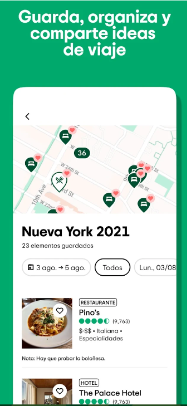
\includegraphics[width=0.32\textwidth]{img/tripadvisor.png} & 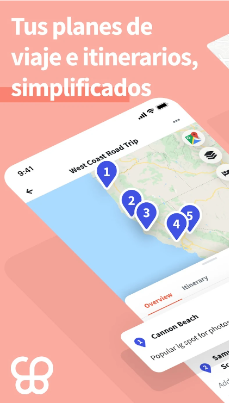
\includegraphics[width=0.34\textwidth]{img/wanderlog.png} \\
	\hline
	\href{https://play.google.com/store/apps/details?id=com.visitacity}{\textbf{Visit A City}} & \href{https://play.google.com/store/apps/details?id=com.tiqets.tiqetsapp}{\textbf{Tiqets - Museos y Atracciones}} \\
	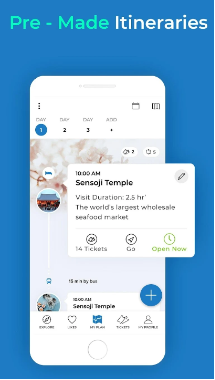
\includegraphics[width=0.35\textwidth]{img/visit_a_city.png} & 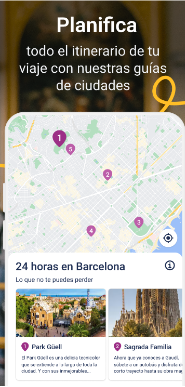
\includegraphics[width=0.31\textwidth]{img/tiquets.png} \\
	\hline
	\end{tabular}
	\caption{Aplicaciones Similares}
	\label{fig:apps_similares}
	\end{table}

\newpage

\begin{table}[h]
	\centering
	\renewcommand{\arraystretch}{1.5} % Controla el espaciado entre las líneas
	\rowcolors{2}{gray!20}{white} % Alterna colores de fondo en las filas
	\begin{tabular}{m{4.5cm} >{\centering\arraybackslash}m{2cm} >{\centering\arraybackslash}m{2cm} >{\centering\arraybackslash}m{2cm} >{\centering\arraybackslash}m{2cm} >{\centering\arraybackslash}m{2.5cm}} % Usamos 'm{<width>}' para centrar verticalmente y ajustamos los anchos
	\toprule
	\textbf{Característica} & \textbf{Tripadvisor} & \textbf{Wanderlog} & \textbf{Visit A City} & \textbf{Tiquets} & \textbf{\textit{Eco City Tour}} \\
	\midrule
	Versión de pago & Sí & Sí & No & No & No\\
	Recomendaciones tienen en cuenta factores de sostenibilidad & No & No & No & No & Sí\\
	Modificación dinámica de rutas & Sí & No & No & No & Sí\\
	Intereses de terceros pueden afectar a los resultados & Sí & Sí & No & No & No \\
	Fuente de datos & Propia & Usuarios - LLM & Usuarios & Propia & LLM\\
	\bottomrule
	\end{tabular}
	\caption{Comparación de aplicaciones similares} % Mueve la leyenda debajo de la tabla
	\label{herramientasportipodeuso}
	\end{table}
\section{Otros \acrfull{tfg}}
	\subsection{Chatbot}
	Trabajo Fin de Carrera de José María Redondo Guerra \cite{chatbot_github} que tuvo como tutores a José Ignacio Santos Martín y Carlos López Nozal.
	
	Este trabajo fue desarrollado usando \acrfull{llm} para la generación de un chat con un sistema \acrshort{rag} para obtener la información de las normas de los \acrshort{tfg} y así mejorar sus respuestas.
	
	\subsection{Visualización de las actividades socioculturales en Castilla y León CULTURALCyL}
	Trabajo Fin de Carrera de Yanela Lozano Pérez con tutores José Ignacio Santos, Virginia Ahedo y Silvia Díaz.
	Esta aplicación mostraba información de eventos culturales para lo cual usaba una aplicación móvil con servicios API.
	Es especialmente interesante como ejemplo de una aplicación móvil con una fuerte característica de usabilidad, ya que se centra en la visualización de mucha información que debe recibir el usuario de manera clara y sencilla.
\capitulo{7}{Conclusiones y Líneas de trabajo futuras}
\section*{Conclusiones}
\section*{Líneas de trabajo futuras}
Existen múltiples maneras de expandir y llenar de nuevas funcionalidades a la aplicación llevada a cabo.
Por citar algunas que puedan resultar más útiles al usuario:
\begin{itemize}
    \item \textbf{Gamificación:} Recompensas por rutas completadas o distancia recorrida con un medio ecológico.
    \item \textbf{Ratings:} Valorar las rutas permitiendo la busqueda de los mismos.
    \item \textbf{Mejora en planificador de rutas:} Determinación de la zona de sombra.
\end{itemize}


\bibliographystyle{plain}
\bibliography{bibliografia}

\end{document}
